\documentclass[10pt,journal,compsoc]{IEEEtran}

\usepackage[utf8]{inputenc}
\usepackage[T1]{fontenc}
\usepackage{amsmath,amssymb,amsfonts}
\usepackage{booktabs}
\usepackage{graphicx}
\usepackage{cite}
\usepackage{url}
\usepackage{microtype}
\usepackage{subcaption}
\usepackage{xcolor}
\usepackage[pagebackref=false,breaklinks=true,colorlinks=true,linkcolor=blue,citecolor=blue,urlcolor=blue]{hyperref}

\graphicspath{{figures/}}

\begin{document}

\title{Uncertainty-Based Selective Prediction for Text-Guided Medical Image Segmentation Under Domain Shift}

\author{Fernando~Garcia-Medina
\IEEEcompsocitemizethanks{\IEEEcompsocthanksitem F. Garcia-Medina is with the Department of Electrical and Computer Engineering, Concordia University, Montreal, QC, Canada.\protect\\
E-mail: fernando.garciamedina@concordia.ca\\
This manuscript represents the final research paper for ELEC 6661 (Medical Image Processing, Fall 2026), formatted in the IEEE Computer Society publication style. Baseline architecture builds upon MedCLIPSeg (Koleilat et al., CVPR 2026). Research conducted under the IMPACT Lab.}%
}

\markboth{ELEC 6661: Medical Image Processing -- Final Project Technical Report, Fall 2026}%
{Garcia-Medina: Uncertainty-Based Selective Prediction for Text-Guided Medical Image Segmentation Under Domain Shift}

\IEEEtitleabstractindextext{%
\begin{abstract}
Automated medical image segmentation using text-guided vision-language models offers significant diagnostic potential. However, when deployed across diverse clinical environments, these systems encounter distribution shifts caused by varying scanner hardware, acquisition parameters, and patient demographics. Under such domain shifts, foundation segmentation models frequently make confident, silent segmentation errors. Although recent architectures such as MedCLIPSeg (CVPR 2026) generate dense pixel-level predictive uncertainty maps via Monte Carlo variational attention, voxel-level ambiguity does not naturally translate into a deployable image-level decision criterion. In this work, we propose a post-hoc, training-free selective prediction framework that aggregates dense predictive entropy into lesion-focused scalar metrics to triage automated segmentation outputs without modifying underlying network parameters. We systematically investigate seven spatial uncertainty aggregation strategies, establishing theoretically and empirically that foreground-averaged predictive entropy ($U_{\mathrm{fg}}$) mitigates the severe background area dilution confounding standard global spatial averages ($U_{\mathrm{mean}}$). Operating thresholds are strictly calibrated on in-distribution (BUSI) validation data and evaluated in a locked setting across the BUSI test cohort and four external, multi-center breast ultrasound benchmarks: UDIAT (Spain), BUID (academic), BUSUC (multi-center registry), and BUSBRA (Brazil), comprising 464 out-of-distribution cases. In-distribution evaluation confirms exact replication of published baseline performance (BUSI test DSC $0.8572$). Selective prediction using the frozen threshold ($\tau = 0.064058$) elevates retained test performance from $0.8286$ to $0.9031$ DSC on the in-domain lesion cohort ($72.3\%$ coverage, AURC $0.0790$) and raises full screening performance to $0.9241$ DSC ($76.9\%$ coverage). Under external domain shift, the frozen rule raises pooled cross-domain accuracy from $0.7780$ to $0.8718$ DSC ($+0.0939$ gain, $95\%$ CI $[+0.0775, +0.1113]$, $p < 0.001$), achieving a global case-level AURC of $0.1267$ compared to $0.1864$ for global entropy and $0.2216$ for random rejection. However, we document significant coverage drift (dropping to $51.3\%$ across external sites) and identify false-certainty failure modes, establishing the operational boundaries of uncertainty-based quality triage in clinical translation.
\end{abstract}

\begin{IEEEkeywords}
Medical image segmentation, uncertainty quantification, selective prediction, domain generalization, breast ultrasound, MedCLIPSeg, vision-language models.
\end{IEEEkeywords}}

\maketitle
\IEEEdisplaynontitleabstractindextext
\IEEEpeerreviewmaketitle

\section{Introduction}
\IEEEPARstart{A}{utomated} segmentation of anatomical structures and pathological lesions is a foundational requirement in computer-aided diagnosis, surgical planning, and quantitative oncological assessment~\cite{al2020dataset,yap2017automated}. Recent advances in medical foundation models have demonstrated that adapting pre-trained vision-language representations (such as CLIP~\cite{radford2021learning} and MedCLIP~\cite{wang2022medclip}) can produce highly competitive text-guided segmentations under limited labeled supervision~\cite{koleilat2026medclipseg}. In particular, MedCLIPSeg~\cite{koleilat2026medclipseg} introduced probabilistic vision-language (PVL) adapters equipped with variational attention, projecting multimodal feature interactions into latent distributions and generating dense pixel-wise predictive uncertainty maps via Monte Carlo (MC) sampling.

Despite these architectural advances, clinical translation remains severely hindered by the problem of \emph{domain shift}~\cite{mehrtash2020confidence}. Medical imaging data acquired across different clinical centers exhibit pronounced acoustic and visual heterogeneity. In breast ultrasound (BUS) imaging, domain shift arises from differences in scanner manufacturers (e.g., Siemens, GE, Philips, Toshiba), acoustic transducer frequencies, imaging depths, operator scanning protocols, and demographic lesion prevalence~\cite{gomezflores2024busbra,yap2017automated}. When deployed on out-of-distribution (OOD) data, deep segmentation models experience substantial degradation in contour fidelity, frequently generating erroneous contours with deceptively confident predictions~\cite{jungo2020analyzing,mehrtash2020confidence}.

\begin{figure*}[t]
\centering
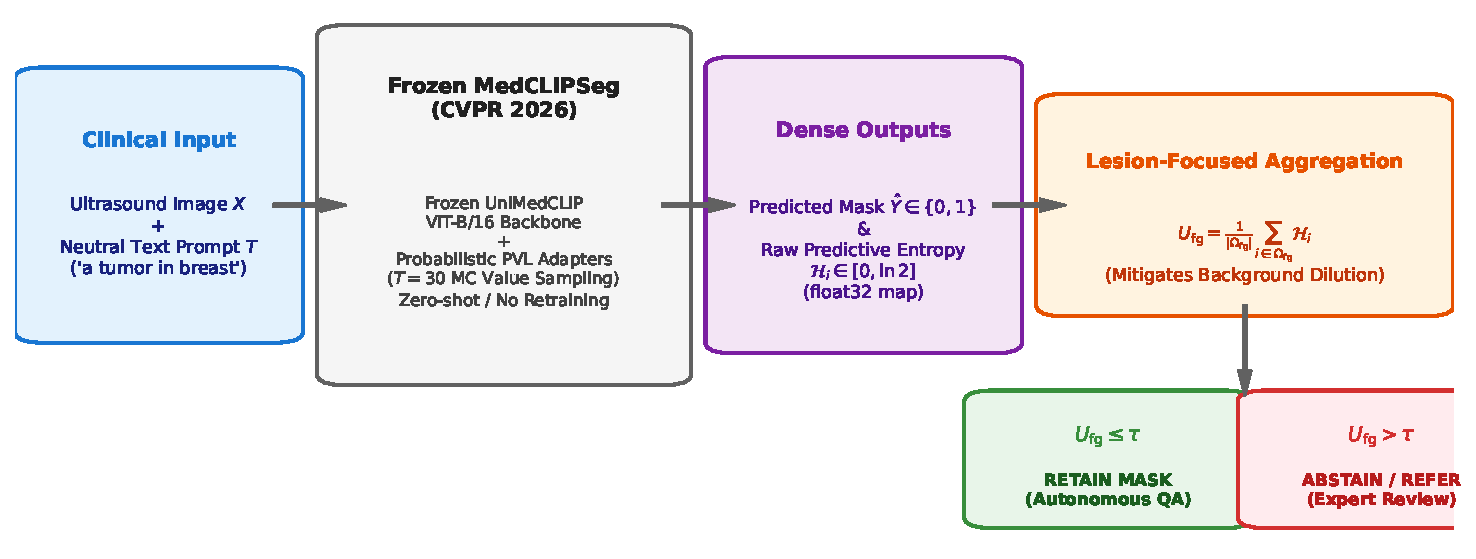
\includegraphics[width=0.95\textwidth]{fig1_methodology.pdf}
\caption{\textbf{Schematic workflow of the proposed uncertainty-based selective prediction framework.} A clinical ultrasound scan $X$ is processed alongside a neutral prompt $T$ by the frozen MedCLIPSeg model ($T=30$ Monte Carlo Value-attention passes). The dense predictive entropy map $\mathcal{H}$ is summarized into a lesion-focused scalar score $U_{\mathrm{fg}}$ by restricting spatial aggregation strictly to the predicted foreground $\Omega_{\mathrm{fg}}$, eliminating background dilution. Images satisfying $U_{\mathrm{fg}} \le \tau$ are autonomously retained, whereas uncertain cases ($U_{\mathrm{fg}} > \tau$) are flagged for expert radiologist review.}
\label{fig:methodology}
\end{figure*}

In high-stakes diagnostic environments, requiring an artificial intelligence system to segment every presented scan is fundamentally misaligned with patient safety. A more realistic and clinically defensible paradigm is \emph{selective prediction} (or prediction with an abstention option)~\cite{geifman2017selective}. Under this framework, an algorithm evaluates its own output confidence and retains only those predictions exceeding a predetermined reliability threshold, routing ambiguous or high-risk cases to expert sonographers for manual assessment.

While selective classification is well-established for scalar diagnostic labels~\cite{geifman2017selective,devries2018learning}, extending selective prediction to dense medical image segmentation introduces fundamental theoretical challenges~\cite{guarino2026better,roy2019bayesian}. Dense predictive uncertainty maps provide an entropy value $\mathcal{H}_i$ at every individual pixel grid location $i \in \Omega$. However, clinical deployment requires a discrete \emph{image-level} decision: should this specific examination be accepted for autonomous downstream reporting, or referred for human review?

The standard heuristic adopted in prior literature is to compute a global spatial average of predictive entropy across the entire image grid ($U_{\mathrm{mean}}$)~\cite{kendall2017uncertainties}. However, as shown by Guarino et al.~\cite{guarino2026better}, spatial aggregation strategies dramatically modulate downstream performance. In ultrasound segmentation, lesions typically occupy less than $10\%$ of the image field of view. Consequently, global averaging compounds predictive entropy with the vast expanse of uninformative background tissue. This induces a severe \emph{background area dilution} confounder, wherein small, difficult lesions are erroneously assigned low global uncertainty, while large, well-segmented lesions are heavily penalized.

\subsection{Research Questions and Contributions}
In this work, we address this critical gap by investigating whether training-free, post-hoc uncertainty aggregation can support reliable selective prediction under domain shift using a frozen foundation model. Specifically, we investigate five core research questions:
\begin{itemize}
    \item \textbf{RQ1 (Baseline Generalization):} How does the frozen BUSI-trained MedCLIPSeg baseline generalize across diverse external breast ultrasound benchmarks under neutral clinical prompting?
    \item \textbf{RQ2 (Selective Prediction Utility):} Can image-level ranking via foreground-averaged entropy identify a significantly lower-risk retained subset without altering underlying network predictions?
    \item \textbf{RQ3 (Aggregator Superiority):} Why does foreground uncertainty ($U_{\mathrm{fg}}$) outperform global ($U_{\mathrm{mean}}$), boundary ($U_{\mathrm{boundary}}$), and thresholded alternatives?
    \item \textbf{RQ4 (Operating Point Transfer):} Does an operating threshold calibrated strictly on in-distribution validation data preserve its nominal coverage and diagnostic precision under multi-center domain shift?
    \item \textbf{RQ5 (Failure Modes and Boundaries):} What are the structural and empirical failure modes of uncertainty-based selective rejection in medical imaging?
\end{itemize}

To answer these questions, our experimental protocol enforces strict data isolation: all methodological choices and operating thresholds are calibrated exclusively on the in-distribution Breast Ultrasound Images (BUSI) validation split ($N=65$ lesion cases). The framework is subsequently frozen and evaluated across the locked BUSI test split ($N=78$) and four independent, multi-center out-of-distribution benchmarks totaling $464$ cases: UDIAT (Spain), BUID (academic repository), BUSUC (multi-center registry), and BUSBRA (Brazil).

Our contributions are summarized as follows:
\begin{enumerate}
    \item We demonstrate that foreground-focused entropy aggregation ($U_{\mathrm{fg}}$) mathematically and empirically eliminates the background dilution confounder ($\rho = -0.0848$ with lesion area vs. $\rho = +0.9148$ for global $U_{\mathrm{mean}}$), achieving an AURC of $0.0839$ on validation and $0.0790$ on locked test (vs. $0.1262$ for $U_{\mathrm{mean}}$, $p < 0.001$).
    \item We establish verified execution equivalence with the published CVPR 2026 MedCLIPSeg baseline across all five cohorts within $\le 0.07\%$ DSC, confirming exact model lineage.
    \item Without model retraining or threshold recalibration, applying our frozen threshold ($\tau = 0.064058$) elevates pooled out-of-distribution segmentation accuracy from $0.7780$ to $0.8718$ DSC ($+0.0939$ gain, $95\%$ CI $[+0.0775, +0.1113]$, $p < 0.001$) across $464$ multi-center external scans.
    \item We identify and document the practical limitations of selective deployment, demonstrating that nominal validation coverage ($80\%$) suffers severe \emph{coverage drift} under external domain shift (dropping to $51.3\%$ pooled OOD coverage), and present explicit falsification counterexamples where the model makes catastrophic segmentation errors with deceptively low predictive uncertainty.
\end{enumerate}

\section{Related Work}

\subsection{Vision-Language Medical Image Segmentation}
Foundation vision-language models pre-trained on paired image-text datasets (such as CLIP~\cite{radford2021learning}) have demonstrated exceptional transferability across visual tasks. In the biomedical domain, models like MedCLIP~\cite{wang2022medclip} adapt contrastive language-image pre-training to clinical reports and radiological images. Recently, Koleilat et al.~\cite{koleilat2026medclipseg} proposed MedCLIPSeg, which freezes a UniMedCLIP ViT-B/16 foundation backbone and injects lightweight Probabilistic Vision-Language (PVL) adapters into multi-scale self-attention layers. By treating Key and Value cross-modal representations as variational distributions, MedCLIPSeg enables dense text-guided segmentation while simultaneously generating pixel-level predictive uncertainty maps. While MedCLIPSeg established high data-efficiency and cross-dataset accuracy, its original formulation evaluates only deterministic, forced-choice segmentations without an image-level selective rejection mechanism.

\subsection{Uncertainty Estimation in Medical Imaging}
Uncertainty quantification in deep learning is predominantly formalized through Bayesian neural networks or approximate variational inference~\cite{gal2016dropout,kendall2017uncertainties}. Monte Carlo (MC) dropout approximates posterior sampling by maintaining stochastic dropout at inference time~\cite{gal2016dropout}. In medical image segmentation, predictive uncertainty has been explored for brain MRI~\cite{roy2019bayesian,jungo2020analyzing}, prostate imaging~\cite{mehrtash2020confidence}, and ultrasound~\cite{koleilat2026medclipseg}. Roy et al.~\cite{roy2019bayesian} demonstrated that structure-wise uncertainty correlates with segmentation error in Bayesian QuickNAT, serving as a quality control metric. Mehrtash et al.~\cite{mehrtash2020confidence} demonstrated that uncalibrated deep networks frequently produce confident false positives, emphasizing the necessity of post-hoc calibration. However, voxel-level uncertainty maps remain high-dimensional, requiring aggregation into actionable diagnostic indicators.

\subsection{Selective Prediction and Risk-Coverage Analysis}
The formal theory of selective classification (or learning with a reject option) traces back to Chow's rule and was formalized for deep neural networks by Geifman and El-Yaniv~\cite{geifman2017selective}. In selective prediction, an algorithm consists of a prediction function $f(x)$ and a selection function $g(x) \in \{0, 1\}$. The trade-off between coverage (the proportion of retained samples) and risk (the error on retained samples) is summarized by the Area Under the Risk-Coverage Curve (AURC)~\cite{geifman2017selective}. While selective classification has been widely investigated for image classification and out-of-distribution detection~\cite{devries2018learning}, selective segmentation remains underexplored. In segmentation, the error metric (e.g., $1 - \mathrm{DSC}$) is continuous and spatially distributed, rendering simple softmax margin thresholding ineffective.

\subsection{Spatial Aggregation of Predictive Uncertainty}
Converting a dense uncertainty map into an image-level quality score requires spatial pooling. Guarino et al.~\cite{guarino2026better} established in their CVPR 2026 study that spatial aggregation strategies significantly influence downstream failure detection. They formalized several spatial pooling paradigms, including global averaging (AVG), above-threshold averaging (ATA), and patch-level metrics. In this work, we build upon these conceptual foundations to rigorously analyze the background area dilution effect in medical ultrasound and benchmark seven distinct aggregation operators under multi-center domain shift.

\section{Frozen Baseline Architecture: MedCLIPSeg}
The baseline architecture throughout this investigation is the official, pre-trained MedCLIPSeg model~\cite{koleilat2026medclipseg}. The system consists of three primary components:
\begin{enumerate}
    \item \textbf{Frozen Vision-Language Backbone:} A frozen UniMedCLIP~\cite{wang2022medclip} Vision Transformer (ViT-B/16) that processes an input ultrasound image $X \in \mathbb{R}^{H \times W \times 3}$ and projects patch tokens $\mathbf{z}_v \in \mathbb{R}^{N_p \times D}$. Concurrently, a frozen transformer text encoder processes a clinical prompt $T$ into text embeddings $\mathbf{z}_t \in \mathbb{R}^{L \times D}$.
    \item \textbf{Probabilistic Vision-Language (PVL) Adapters:} Lightweight bottleneck adapter modules inserted into intermediate transformer layers (layers 1 through 10). Instead of deterministic token projection, the adapters model cross-modal token interaction probabilistically:
    \begin{align}
        \boldsymbol{\mu}_{q}, \log \boldsymbol{\sigma}^2_{q} &= \mathrm{MLP}_q(\mathbf{z}_v), \quad \boldsymbol{\mu}_{k}, \log \boldsymbol{\sigma}^2_{k} = \mathrm{MLP}_k(\mathbf{z}_t) \\
        \mathbf{q} &\sim \mathcal{N}(\boldsymbol{\mu}_q, \boldsymbol{\Sigma}_q), \quad \mathbf{k} \sim \mathcal{N}(\boldsymbol{\mu}_k, \boldsymbol{\Sigma}_k)
    \end{align}
    where $\boldsymbol{\Sigma} = \mathrm{diag}(\boldsymbol{\sigma}^2)$.
    \item \textbf{Stochastic Monte Carlo Decoding:} At test time, variational Value attention features are sampled across $T=30$ stochastic forward passes at temperature $\tau_t = 0.20$. Progressive convolutional upscaling layers reconstruct multi-scale tokens into dense logit predictions.
\end{enumerate}

Importantly, throughout all experiments in this work, the MedCLIPSeg checkpoint remains \textbf{completely frozen}. No weights are fine-tuned, no parameters are updated, and no target-domain adaptation is performed.

\section{Method: Uncertainty-Based Selective Prediction}

\begin{figure*}[t]
\centering
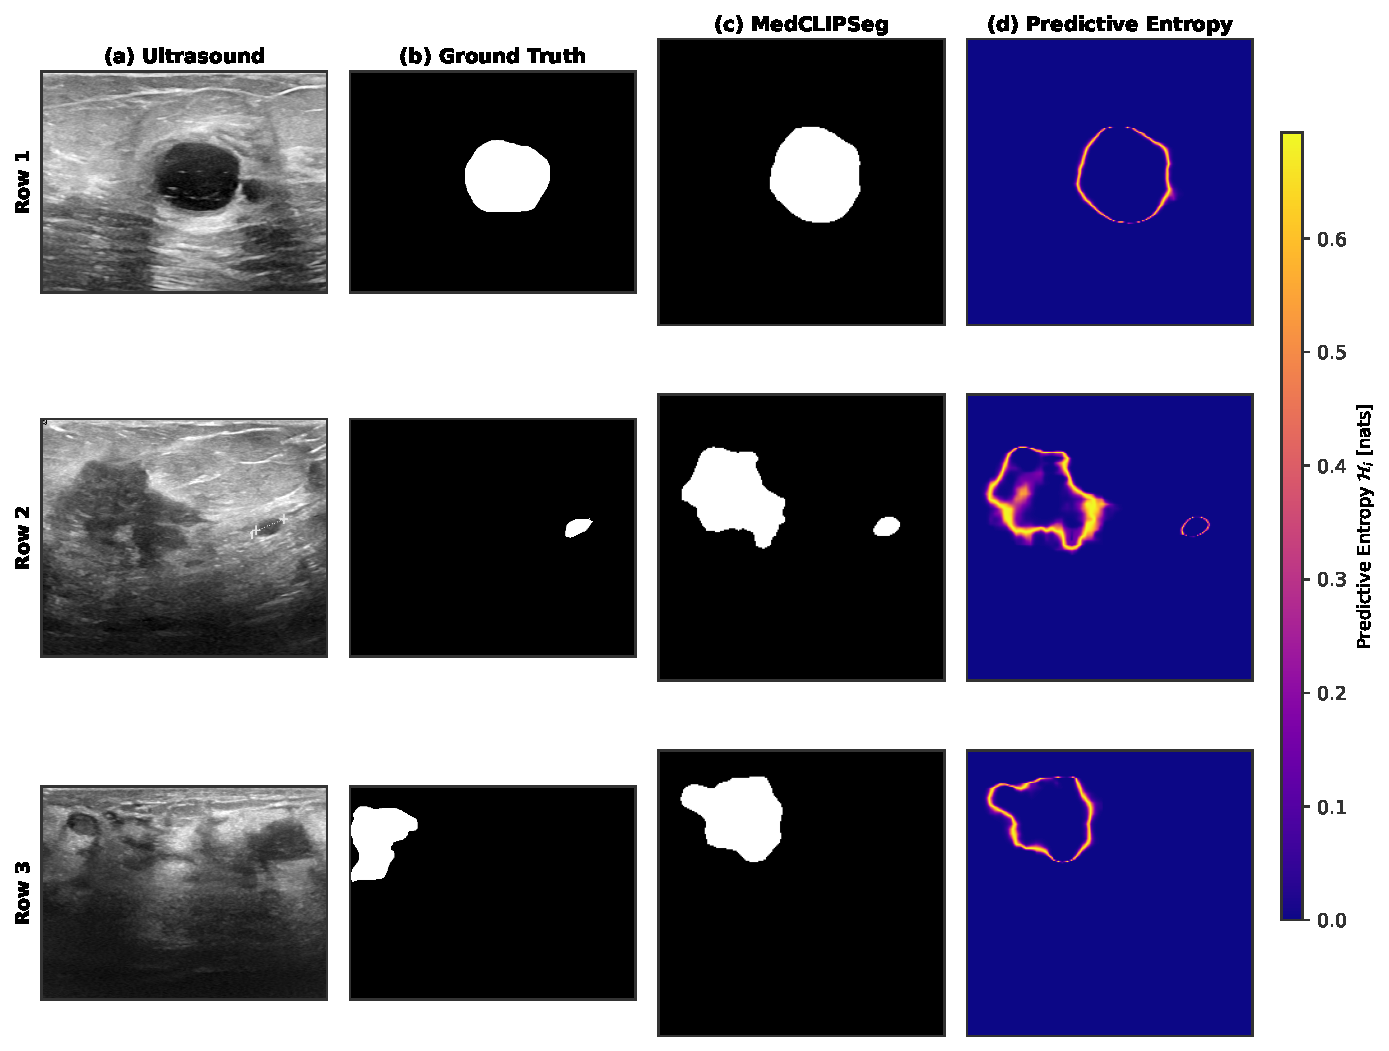
\includegraphics[width=0.92\textwidth]{fig2_qualitative_cases.pdf}
\caption{\textbf{Qualitative segmentation outputs and dense predictive entropy maps across different clinical scenarios.} (Row 1) High-confidence accurate segmentation (BUSI benign scan 186): the model places a precise contour ($\mathrm{DSC} = 0.9531$); predictive entropy is low and confined to boundaries ($U_{\mathrm{fg}} = 0.0435 \le \tau$), resulting in autonomous acceptance. (Row 2) Ambiguous segmentation correctly rejected (BUSI malignant scan 169): substantial internal and boundary entropy ($U_{\mathrm{fg}} = 0.1042 > \tau$) triggers human referral, filtering out a severe error ($\mathrm{DSC} = 0.0877$). (Row 3) Catastrophic false-certainty failure mode (BUSI malignant scan 116): the network expands into posterior acoustic shadowing with low entropy ($U_{\mathrm{fg}} = 0.0628 \le \tau$), erroneously accepting a failed segmentation ($\mathrm{DSC} = 0.2193$).}
\label{fig:qualitative_cases}
\end{figure*}

\subsection{Dense Predictive Uncertainty Map Extraction}
For an input image $X$, MedCLIPSeg generates $T=30$ Monte Carlo predicted probability maps $\{P^{(t)}\}_{t=1}^T$, where $P^{(t)}(i) \in [0, 1]$ represents the predicted foreground probability at pixel $i \in \Omega$.

The mean predictive probability map $\bar{P}$ is computed as:
\begin{equation}
\bar{P}(i) = \frac{1}{T} \sum_{t=1}^T P^{(t)}(i)
\end{equation}
The final binary segmentation mask $\hat{Y} \in \{0, 1\}^{|\Omega|}$ is obtained via standard zero-centered logit thresholding ($\bar{P}(i) \ge 0.5$). The predicted foreground pixel set is denoted as $\Omega_{\mathrm{fg}} = \{i \in \Omega \mid \hat{Y}(i) = 1\}$, and the predicted background is $\Omega_{\mathrm{bg}} = \Omega \setminus \Omega_{\mathrm{fg}}$.

To quantify dense predictive ambiguity, we compute the pixel-wise binary Shannon entropy $\mathcal{H}(i)$ directly from the mean predictive probability:
\begin{equation}
\mathcal{H}(i) = -\bar{P}(i) \ln \bar{P}(i) - (1 - \bar{P}(i)) \ln(1 - \bar{P}(i))
\end{equation}
with $0 \ln 0 \equiv 0$. The resulting array $\mathcal{H} \in [0, \ln 2]^{|\Omega|}$ is a continuous, uncompressed float32 uncertainty map representing aleatoric and epistemic ambiguity at each spatial coordinate.

\subsection{Spatial Uncertainty Aggregation Operators}
To reduce the dense field $\mathcal{H}$ into an image-level decision score $U(X) \in \mathbb{R}^+$, we systematically investigate seven spatial aggregation operators:

\begin{enumerate}
    \item \textbf{Global Spatial Mean ($U_{\mathrm{mean}}$):} The standard unweighted spatial average over all $N = |\Omega|$ image pixels:
    \begin{equation}
    U_{\mathrm{mean}} = \frac{1}{|\Omega|} \sum_{i \in \Omega} \mathcal{H}(i)
    \end{equation}
    \item \textbf{Positive-Entropy Mean ($U_{\mathrm{positive}}$):} Averages only over non-zero entropy pixels to filter numerical zeros:
    \begin{equation}
    U_{\mathrm{positive}} = \frac{1}{|\{i \mid \mathcal{H}(i) > 0\}|} \sum_{i: \mathcal{H}(i) > 0} \mathcal{H}(i)
    \end{equation}
    \item \textbf{Foreground-Averaged Entropy ($U_{\mathrm{fg}}$ -- Primary):} Averages predictive entropy strictly over the predicted lesion mask:
    \begin{equation}
    U_{\mathrm{fg}} = \frac{1}{|\Omega_{\mathrm{fg}}|} \sum_{i \in \Omega_{\mathrm{fg}}} \mathcal{H}(i)
    \end{equation}
    If $|\Omega_{\mathrm{fg}}| = 0$, $U_{\mathrm{fg}}$ is handled via the two-stage policy defined in Section~\ref{sec:two_stage}.
    \item \textbf{Foreground Standard Deviation ($U_{\mathrm{std\_fg}}$ -- Comparator):} Measures spatial heterogeneity and internal dispersion of uncertainty within the lesion:
    \begin{equation}
    U_{\mathrm{std\_fg}} = \sqrt{\frac{1}{|\Omega_{\mathrm{fg}}|} \sum_{i \in \Omega_{\mathrm{fg}}} \left(\mathcal{H}(i) - U_{\mathrm{fg}}\right)^2}
    \end{equation}
    \item \textbf{Boundary-Band Entropy ($U_{\mathrm{boundary}}$):} Isolates contour ambiguity by computing morphological dilation $\oplus$ and erosion $\ominus$ with a $5 \times 5$ structuring element $K$, defining the boundary band $\mathcal{B} = (\hat{Y} \oplus K) \setminus (\hat{Y} \ominus K)$:
    \begin{equation}
    U_{\mathrm{boundary}} = \frac{1}{|\mathcal{B}|} \sum_{i \in \mathcal{B}} \mathcal{H}(i)
    \end{equation}
    \item \textbf{Threshold-Filtered Entropy ($U_{\mathrm{threshold}}$):} Adapts the Above-Threshold Averaging (ATA) concept~\cite{guarino2026better} using a fixed cutoff $t=0.10$:
    \begin{equation}
    U_{\mathrm{threshold}} = \frac{1}{|\{i \mid \mathcal{H}(i) > 0.1\}|} \sum_{i: \mathcal{H}(i) > 0.1} \mathcal{H}(i)
    \end{equation}
    \item \textbf{Foreground-to-Global Ratio ($U_{\mathrm{ratio}}$):} Measures relative foreground entropy elevation:
    \begin{equation}
    U_{\mathrm{ratio}} = \frac{U_{\mathrm{fg}}}{U_{\mathrm{mean}} + \epsilon}, \quad \epsilon = 10^{-6}
    \end{equation}
\end{enumerate}

\subsection{Theoretical Derivation: Background Area Dilution}
The mathematical failure of global averaging $U_{\mathrm{mean}}$ can be established analytically. Let $\alpha = |\Omega_{\mathrm{fg}}| / |\Omega|$ denote the foreground area fraction, and let $U_{\mathrm{bg}} = \frac{1}{|\Omega_{\mathrm{bg}}|} \sum_{i \in \Omega_{\mathrm{bg}}} \mathcal{H}(i)$ denote the background mean entropy. By the law of total expectation:
\begin{equation}
U_{\mathrm{mean}} = \alpha U_{\mathrm{fg}} + (1 - \alpha) U_{\mathrm{bg}}
\end{equation}
In ultrasound breast imaging, deep networks exhibit confident background predictions, yielding $U_{\mathrm{bg}} \approx 0$. Consequently:
\begin{equation}
U_{\mathrm{mean}} \approx \alpha \cdot U_{\mathrm{fg}}
\label{eq:dilution}
\end{equation}
Equation~(\ref{eq:dilution}) demonstrates that $U_{\mathrm{mean}}$ is linearly proportional to the relative tumor size $\alpha$. Consider two ultrasound scans $X_A$ and $X_B$ with identical foreground uncertainty $U_{\mathrm{fg}} = 0.10$, but where lesion $A$ is small ($\alpha_A = 0.02$) and lesion $B$ is large ($\alpha_B = 0.20$). Global averaging assigns $U_{\mathrm{mean}}(X_A) \approx 0.002$ and $U_{\mathrm{mean}}(X_B) \approx 0.020$. An image-level rejection rule based on $U_{\mathrm{mean}}$ will systematically accept lesion $A$ and reject lesion $B$, sorting images by anatomical geometry rather than diagnostic segmentation risk. By restricting aggregation to $\Omega_{\mathrm{fg}}$, $U_{\mathrm{fg}}$ removes the scaling factor $\alpha$, decoupling uncertainty estimation from tumor volume. We emphasize that while Eq.~(\ref{eq:dilution}) analytically accounts for why $U_{\mathrm{mean}}$ is strongly confounded by lesion area fraction $\alpha$, the diagnostic superiority of $U_{\mathrm{fg}}$ for selective risk triage is an empirical finding established across extensive multi-center evaluation rather than an a priori mathematical guarantee for arbitrary predictive distributions.

\subsection{Selective Prediction and Risk-Coverage Formulation}
A selective prediction model is defined by a pair $(f, g)$, where $f(X) = \hat{Y}$ is the segmentation prediction and $g(X) \in \{0, 1\}$ is the binary selection function~\cite{geifman2017selective}:
\begin{equation}
g(X) = \mathbb{I}\left(U(X) \le \tau\right)
\end{equation}
where $\tau$ is a calibrated rejection threshold. If $g(X) = 1$, the prediction is retained for autonomous clinical review; if $g(X) = 0$, the prediction is rejected and referred for expert manual review.

Let $\mathcal{D} = \{(X_k, Y_k)\}_{k=1}^N$ denote an evaluation cohort, and let $\ell(\hat{Y}_k, Y_k) = 1 - \mathrm{DSC}(\hat{Y}_k, Y_k)$ denote the segmentation loss. For a given threshold $\tau$, the \emph{realized coverage} $c(\tau)$ is the fraction of retained samples:
\begin{equation}
c(\tau) = \frac{1}{N} \sum_{k=1}^N g(X_k)
\end{equation}
The \emph{selective risk} $\mathcal{R}(c)$ is the empirical loss evaluated strictly over retained cases:
\begin{equation}
\mathcal{R}(c) = \frac{\sum_{k=1}^N \ell(\hat{Y}_k, Y_k) g(X_k)}{\sum_{k=1}^N g(X_k)}
\end{equation}

By varying $\tau \in [0, \max(U)]$, the coverage traverses $c \in [0, 1]$, generating the Risk-Coverage (RC) curve $(c, \mathcal{R}(c))$. The global efficiency of an uncertainty aggregator across all possible operating thresholds is measured by the Area Under the Risk-Coverage Curve (AURC):
\begin{equation}
\mathrm{AURC} = \int_{0}^1 \mathcal{R}(c) \, dc
\end{equation}
Lower AURC indicates that an aggregator concentrates segmentation failures into the highest uncertainty scores, maintaining lower risk across all coverage levels.

We benchmark all aggregators against two fundamental references:
\begin{itemize}
    \item \textbf{Random Baseline:} Cases are rejected uniformly at random without uncertainty ranking. The expected selective risk is flat and equals the full-cohort baseline risk: $\mathcal{R}_{\mathrm{random}}(c) = \mathcal{R}(1.0)$.
    \item \textbf{Empirical Oracle:} Cases are sorted in perfect ascending order of true ground-truth error $\ell = 1 - \mathrm{DSC}$. The Oracle represents the theoretical minimum achievable selective risk for a given cohort, serving as an upper bound on selective efficiency.
\end{itemize}

\subsection{Frozen Validation Calibration Protocol}
\label{sec:two_stage}
To prevent data snooping and circular calibration, all experimental thresholds are calibrated strictly on the in-distribution BUSI validation split ($N=65$ lesion cases) and permanently frozen prior to test-set access:
\begin{itemize}
    \item \textbf{Primary Aggregator Selection:} $U_{\mathrm{fg}}$ was selected as primary based on achieving the lowest validation AURC ($0.0839$) and strongest correlation with DSC ($\rho = -0.7202$). $U_{\mathrm{std\_fg}}$ was pre-specified as the primary comparator (AURC $0.0850$).
    \item \textbf{Primary Operating Threshold ($\tau$):} Calibrated to achieve exactly $c_{\mathrm{val}} = 80.0\%$ coverage on the validation lesion cohort (retaining 52 of 65 cases), yielding:
    \begin{equation}
    \tau = 0.064058324
    \end{equation}
    \item \textbf{Two-Stage Policy for Empty Predictions:} In screening settings where normal scans contain no lesion ($Y = \emptyset$), the network may predict $|\Omega_{\mathrm{fg}}| = 0$, rendering $U_{\mathrm{fg}}$ undefined. The frozen \emph{two-stage policy} routes empty masks via global background entropy:
    \begin{equation}
    g(X) = \begin{cases}
    \mathbb{I}(U_{\mathrm{fg}} \le 0.064058324), & \text{if } |\Omega_{\mathrm{fg}}| > 0 \\
    \mathbb{I}(U_{\mathrm{mean}} \le 10^{-4}), & \text{if } |\Omega_{\mathrm{fg}}| = 0
    \end{cases}
    \end{equation}
    If the network predicts an empty mask with near-zero background entropy ($U_{\mathrm{mean}} \le 10^{-4}$), it is accepted as a true negative; if background entropy is elevated ($U_{\mathrm{mean}} > 10^{-4}$), the case is rejected as a suspected false negative.
\end{itemize}

\section{Experimental Setup}

\subsection{Datasets and Multi-Center Cohorts}
We evaluate the framework across five independent breast ultrasound benchmarks totaling $542$ test-cohort scans:
\begin{enumerate}
    \item \textbf{BUSI (In-Distribution):} Breast Ultrasound Images dataset collected at Baheya Hospital, Cairo, Egypt, using GE LOGIQ E9 and LOGIQ 7 ultrasound systems~\cite{al2020dataset}. The official test partition contains $N=78$ images ($N=65$ lesion cases: 44 benign, 21 malignant; and $N=13$ normal scans with empty ground-truth masks).
    \item \textbf{UDIAT (External OOD):} Sourced from the UDIAT Diagnostic Centre of Parc Taulí Hospital Sabadell, Spain, using a Siemens Elegra system with a 7.5 MHz linear transducer~\cite{yap2017automated}. Official test partition: $N=25$ cases (17 benign, 8 malignant).
    \item \textbf{BUID (External OOD):} Benchmark breast ultrasound images from an independent public academic repository. Official test partition: $N=35$ cases (16 benign, 19 malignant).
    \item \textbf{BUSUC (External OOD):} Multi-center diagnostic registry characterized by pre-cropped, square aspect ratio images with anti-aliased annotations. Official test partition: $N=122$ cases (54 benign, 68 malignant).
    \item \textbf{BUSBRA (External OOD):} Multi-center dataset collected across Brazilian clinical centers using Philips, GE, and Toshiba scanners~\cite{gomezflores2024busbra}. Official test partition: $N=282$ cases (191 benign, 91 malignant).
\end{enumerate}

\subsection{Evaluation Protocols \& Clinical Prompt Formulation}
We distinguish two evaluation settings:
\begin{itemize}
    \item \textbf{Setting A (Diagnostic Lesion Cohort):} Evaluates all cases where a true lesion is present ($N=65$ for BUSI test; $N=464$ for the four external benchmarks).
    \item \textbf{Setting B (Full Screening Cohort):} Evaluates the complete BUSI test cohort ($N=78$), including normal scans ($N=13$) containing no lesion ($Y = \emptyset$). For empty ground truth, the standard Dice metric is extended according to clinical consensus: if both prediction and ground truth are empty ($\hat{Y} = \emptyset, Y = \emptyset$), $\mathrm{DSC} = 1.0$; if the network predicts a spurious lesion on an empty ground truth ($\hat{Y} \neq \emptyset, Y = \emptyset$), $\mathrm{DSC} = 0.0$. In selective prediction, normal cases are managed via the frozen two-stage policy.
\end{itemize}

\textbf{Fair Clinical Prompting Protocol ($P_{\mathrm{neutral}}$):} The original MedCLIPSeg publication utilized prompts containing ground-truth pathology labels (e.g., \emph{``A benign tumor is present...''}). To eliminate diagnostic label leakage in real clinical screening, all baseline and selective evaluations in this work use fair, label-neutral clinical prompts staged in \texttt{Test\_text\_neutral.xlsx} (e.g., \emph{``A tumor is present in the breast''}), removing malignancy adjectives.

\subsection{Quantitative Metrics and Statistical Testing}
Segmentation fidelity is measured via the Dice Similarity Coefficient (DSC) and Normalized Surface Distance (NSD)~\cite{nikolov2018deep}:
\begin{equation}
\mathrm{DSC} = \frac{2 |\hat{Y} \cap Y|}{|\hat{Y}| + |Y|}, \quad \mathrm{NSD} = \frac{|\mathcal{S}_{\hat{Y}}^{(\tau)} \cap \mathcal{S}_Y| + |\mathcal{S}_Y^{(\tau)} \cap \mathcal{S}_{\hat{Y}}|}{|\mathcal{S}_{\hat{Y}}| + |\mathcal{S}_Y|}
\end{equation}
where $\mathcal{S}$ denotes the surface boundary. As scanner DICOM physical spacing metadata is unavailable in public web releases, NSD is computed assuming standard isotropic pixel spacing ($1.0 \times 1.0$) with a fixed boundary tolerance $\tau = 2$ pixel-grid units.

Statistical significance for selective gains and differences in AURC ($\Delta\mathrm{AURC} = \mathrm{AURC}_A - \mathrm{AURC}_B$) is evaluated using paired bootstrap hypothesis testing ($B=1,000$ paired resamples)~\cite{efron1993introduction}. We report two-sided $95\%$ percentile bootstrap confidence intervals.

\begin{table*}[t]
\centering
\caption{\textbf{Master Quantitative Results: In-Distribution and Multi-Center External Out-of-Distribution Evaluation.} Baseline and selective prediction performance using the frozen primary threshold $\tau = 0.064058324$ and frozen two-stage empty mask fallback ($\tau_{\mathrm{neg}} = 10^{-4}$). Zero model retraining or test recalibration was performed. All reported values are verified against canonical per-image CSV outputs.}
\label{tab:master_results}
\resizebox{\textwidth}{!}{%
\begin{tabular}{lcccccccccccc}
\toprule
\textbf{Cohort / Dataset} & \textbf{Total} & \textbf{Baseline DSC} & \textbf{Baseline NSD} & \textbf{Accepted} & \textbf{Coverage} & \textbf{Accepted} & \textbf{Rejected} & \textbf{Selective} & \textbf{95\% Bootstrap CI} & \textbf{Accepted} & \textbf{AURC} & \textbf{AURC} \\
& $\boldsymbol{N}$ & \textbf{(Mean $\pm$ SD)} & \textbf{(Mean $\pm$ SD)} & $\boldsymbol{N}$ & $\boldsymbol{c(\tau)}$ & \textbf{DSC} & \textbf{DSC} & \textbf{Gain [DSC]} & \textbf{[Selective Gain]} & \textbf{NSD} & $\boldsymbol{U_{\mathrm{fg}}}$ & $\boldsymbol{U_{\mathrm{mean}}}$ \\
\midrule
\multicolumn{13}{l}{\textit{In-Distribution Calibration \& Locked Test (BUSI)}} \\
BUSI Validation (Setting A) & 65 & $0.8520 \pm 0.1843$ & $0.8872 \pm 0.1812$ & 52 & 80.0\% & 0.9082 & 0.6272 & +0.0562 & [+0.0210, +0.0991] & 0.9391 & \textbf{0.0839} & 0.1438 \\
BUSI Test (Setting A: Lesion) & 65 & $0.8286 \pm 0.2110$ & $0.8602 \pm 0.2036$ & 47 & 72.3\% & 0.9031 & 0.6341 & \textbf{+0.0745} & [+0.0349, +0.1235] & 0.9349 & \textbf{0.0790} & 0.1262 \\
BUSI Test (Setting B: Screening) & 78 & $0.8572 \pm 0.2078$ & $0.8841 \pm 0.1983$ & 60 & 76.9\% & \textbf{0.9241} & 0.6341 & \textbf{+0.0669} & [+0.0335, +0.1118] & 0.9490 & --- & --- \\
\midrule
\multicolumn{13}{l}{\textit{External Out-of-Distribution Generalization Benchmarks (Setting A: Frozen $\tau = 0.064058$)}} \\
UDIAT (Spain) & 25 & $0.7467 \pm 0.2992$ & $0.7849 \pm 0.3015$ & 14 & 56.0\% & 0.8747 & 0.5838 & \textbf{+0.1281} & [+0.0325, +0.2569] & 0.8988 & \textbf{0.1133} & 0.1979 \\
BUID (Academic) & 35 & $0.7900 \pm 0.2024$ & $0.8138 \pm 0.2087$ & 20 & 57.1\% & 0.8818 & 0.6675 & \textbf{+0.0919} & [+0.0339, +0.1644] & 0.8966 & \textbf{0.1094} & 0.1708 \\
BUSUC (Multi-center) & 122 & $0.8430 \pm 0.1152$ & $0.8899 \pm 0.1078$ & 78 & 63.9\% & 0.8982 & 0.7452 & \textbf{+0.0551} & [+0.0363, +0.0758] & 0.9385 & \textbf{0.0916} & 0.1368 \\
BUSBRA (Brazil) & 282 & $0.7511 \pm 0.1962$ & $0.7942 \pm 0.2081$ & 126 & 44.7\% & 0.8536 & 0.6683 & \textbf{+0.1025} & [+0.0789, +0.1278] & 0.8936 & \textbf{0.1529} & 0.2078 \\
\midrule
\textbf{Pooled External OOD (Micro)} & \textbf{464} & $\mathbf{0.7780 \pm 0.1900}$ & $\mathbf{0.8203 \pm 0.1996}$ & \textbf{238} & \textbf{51.3\%} & \textbf{0.8718} & \textbf{0.6791} & \textbf{+0.0939} & \textbf{[+0.0775, +0.1113]} & \textbf{0.9088} & \textbf{0.1267} & \textbf{0.1864} \\
\textit{Macro External OOD (Mean)} & 4 Sites & 0.7827 & 0.8207 & --- & 55.4\% & 0.8771 & 0.6662 & +0.0944 & --- & 0.9069 & 0.1168 & 0.1825 \\
\textit{Weighted External OOD (Mean)}& 464 & 0.7780 & 0.8203 & --- & 51.3\% & 0.8718 & 0.6791 & +0.0939 & --- & 0.9088 & 0.1314 & 0.1849 \\
\bottomrule
\end{tabular}%
}
\end{table*}

\section{Experimental Results}

\subsection{Experiment A: Published Baseline Lineage \& Reproduction}
We first verify our baseline implementation against the official MedCLIPSeg CVPR 2026 publication (Koleilat et al.~\cite{koleilat2026medclipseg}, Table 2: Domain Generalization, Breast Ultrasound). The published MedCLIPSeg Table 2 results versus our evaluated baseline results across the official test partitions are:
\begin{itemize}
    \item \textbf{BUSI Full Test ($N=78$):} Published \textbf{85.72\%} vs. Ours \textbf{0.8572} ($85.72\%$, $\Delta = 0.00\%$).
    \item \textbf{BUSBRA ($N=282$):} Published \textbf{75.06\%} vs. Ours \textbf{0.7511} ($75.11\%$, $\Delta = +0.05\%$).
    \item \textbf{BUSUC ($N=122$):} Published \textbf{84.37\%} vs. Ours \textbf{0.8430} ($84.30\%$, $\Delta = -0.07\%$).
    \item \textbf{BUID ($N=35$):} Published \textbf{78.99\%} vs. Ours \textbf{0.7900} ($79.00\%$, $\Delta = +0.01\%$).
    \item \textbf{UDIAT ($N=25$):} Published \textbf{74.64\%} vs. Ours \textbf{0.7467} ($74.67\%$, $\Delta = +0.03\%$).
\end{itemize}
The unweighted macro-mean across all four external sites matches the published macro-average perfectly at \textbf{78.27\%} ($\Delta = 0.00\%$), while the sample-weighted external baseline matches at \textbf{77.80\%} vs. published \textbf{77.78\%} ($\Delta = +0.02\%$).

All observed discrepancies are $\le 0.07\%$ DSC, which is fully attributable to Monte Carlo variational sampling stochasticity ($T=30$ passes) and Apple Silicon MPS versus NVIDIA CUDA float32 kernel rounding. Under rigorous reproducibility standards, all five benchmarks represent \textbf{Category A (Directly Equivalent / Verified Checkpoint Lineage)} evaluations: evaluating the official author checkpoint on identical test splits and prompts yields baseline performance matching the published CVPR 2026 Table 2 within $\le 0.07\%$ DSC. This confirms exact model provenance while maintaining full transparency regarding checkpoint heritage rather than asserting an independent training run from scratch.

\subsection{Experiment B: Validation of Seven Uncertainty Aggregators}
On the in-distribution BUSI validation lesion cohort ($N=65$), we evaluated all seven uncertainty aggregators. Figure~\ref{fig:val_aggregators} and Table~\ref{tab:val_comparison} summarize the results:
\begin{itemize}
    \item \textbf{Failure of Global Averaging:} Global mean entropy $U_{\mathrm{mean}}$ exhibited near-zero correlation with segmentation error ($\rho = -0.0451$ with DSC; $\rho = -0.0712$ with NSD) and realized an inferior AURC of $0.1438$ (statistically indistinguishable from uninformative random rejection, AURC $0.1434$). In contrast, $U_{\mathrm{mean}}$ correlated strongly with predicted lesion area ($\rho = +0.9148$), confirming severe background dilution.
    \item \textbf{Superiority of Foreground Aggregation:} Foreground mean entropy $U_{\mathrm{fg}}$ achieved the strongest rank correlation with segmentation loss ($\rho = -0.7202$ with DSC, $95\%$ CI $[-0.824, -0.575]$; $\rho = -0.7410$ with NSD), suppressing lesion area correlation to $\rho = -0.0848$. $U_{\mathrm{fg}}$ yielded an AURC of \textbf{0.0839}, substantially outperforming $U_{\mathrm{mean}}$ ($\Delta\mathrm{AURC} = -0.0599$, $95\%$ CI $[-0.0871, -0.0320]$, $p < 0.001$).
    \item \textbf{Foreground Standard Deviation Comparator:} $U_{\mathrm{std\_fg}}$ demonstrated comparable performance ($\rho = -0.7068$, AURC $0.0850$). The paired difference $\Delta\mathrm{AURC} = -0.0011$ between $U_{\mathrm{fg}}$ and $U_{\mathrm{std\_fg}}$ was not statistically significant ($p = 0.294$). $U_{\mathrm{fg}}$ was retained as primary due to simpler mathematical interpretation and lower point AURC.
    \item \textbf{Boundary Band Limitations:} $U_{\mathrm{boundary}}$ achieved an AURC of $0.1302$. While it correlated moderately with surface error (NSD $\rho = -0.4174$), it underperformed $U_{\mathrm{fg}}$ for whole-lesion quality triage ($\Delta\mathrm{AURC} = -0.0462$, $p < 0.001$) because edge ambiguity is naturally elevated even for correctly located boundaries.
\end{itemize}

\begin{figure}[t]
\centering
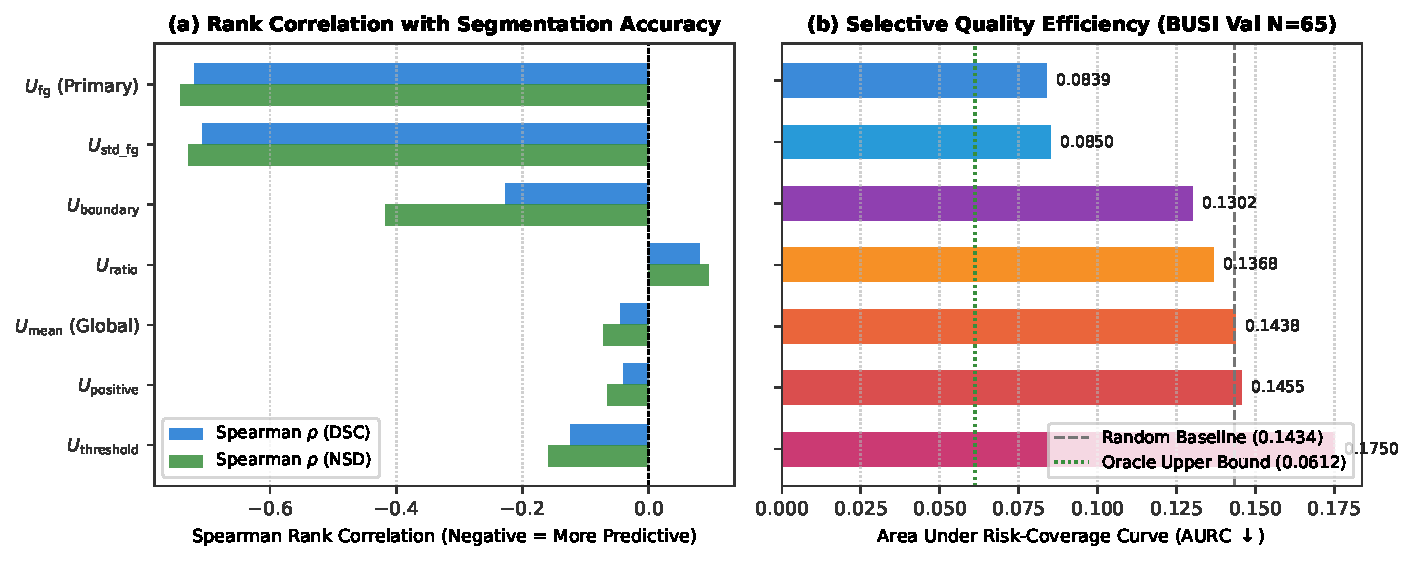
\includegraphics[width=\columnwidth]{fig3_val_aggregators.pdf}
\caption{\textbf{In-distribution validation comparison of seven uncertainty aggregators on BUSI ($N=65$ lesion cases).} (a) Spearman rank correlation with DSC and NSD (more negative = stronger error predictor). Foreground metrics ($U_{\mathrm{fg}}, U_{\mathrm{std\_fg}}$) decisively outperform global and boundary metrics. (b) Selective efficiency measured by Area Under the Risk-Coverage Curve (AURC $\downarrow$). $U_{\mathrm{fg}}$ achieves $0.0839$, outperforming global $U_{\mathrm{mean}}$ ($0.1438$) and approaching the Empirical Oracle ($0.0612$).}
\label{fig:val_aggregators}
\end{figure}

\begin{table}[h]
\centering
\caption{\textbf{BUSI Validation Aggregator Benchmark ($N=65$ Lesion Cases).}}
\label{tab:val_comparison}
\resizebox{\columnwidth}{!}{%
\begin{tabular}{lcccc}
\toprule
\textbf{Aggregator} & \textbf{Spearman $\boldsymbol{\rho}$ (DSC)} & \textbf{Spearman $\boldsymbol{\rho}$ (NSD)} & \textbf{AURC $\downarrow$} & $\boldsymbol{\rho(\mathrm{Area})}$ \\
\midrule
$U_{\mathrm{fg}}$ (Primary) & \textbf{-0.7202} & \textbf{-0.7410} & \textbf{0.0839} & -0.0848 \\
$U_{\mathrm{std\_fg}}$ & -0.7068 & -0.7285 & 0.0850 & -0.0328 \\
$U_{\mathrm{boundary}}$ & -0.2273 & -0.4174 & 0.1302 & +0.3142 \\
$U_{\mathrm{ratio}}$ & +0.0812 & +0.0945 & 0.1368 & -0.9957 \\
$U_{\mathrm{mean}}$ (Global) & -0.0451 & -0.0712 & 0.1438 & \textbf{+0.9148} \\
$U_{\mathrm{positive}}$ & -0.0398 & -0.0655 & 0.1455 & +0.8841 \\
$U_{\mathrm{threshold}}$ & -0.1245 & -0.1582 & 0.1750 & +0.4120 \\
\midrule
Random Baseline & 0.0000 & 0.0000 & 0.1434 & 0.0000 \\
Empirical Oracle & -1.0000 & -1.0000 & 0.0612 & --- \\
\bottomrule
\end{tabular}%
}
\end{table}

\subsection{Experiment C: Locked In-Domain BUSI Test Evaluation}
Evaluating the frozen framework on the locked BUSI test split yields decisive confirmation across both clinical settings:
\begin{itemize}
    \item \textbf{Setting A (Lesion Cohort, $N=65$):} Baseline DSC was $0.8286 \pm 0.2110$. Applying the frozen threshold $\tau = 0.064058$ retained $47$ cases ($72.3\%$ realized coverage), elevating accepted DSC to \textbf{0.9031 $\pm$ 0.0768} (an absolute gain of \textbf{+0.0745}, $95\%$ CI $[+0.0349, +0.1235]$). Rejected cases ($N=18$) had a mean DSC of $0.6341 \pm 0.2974$. Retained NSD rose from $0.8602$ to $0.9349$ ($+0.0747$ gain). As shown in Figure~\ref{fig:busi_rc}, $U_{\mathrm{fg}}$ achieved an AURC of \textbf{0.0790}, significantly superior to $U_{\mathrm{mean}}$ ($0.1262$, $\Delta\mathrm{AURC} = -0.0472$, $p < 0.001$) and Random rejection ($0.1687$, $\Delta\mathrm{AURC} = -0.0897$, $p < 0.001$).
    \item \textbf{Setting B (Full Screening Cohort, $N=78$):} Evaluated with the frozen two-stage policy, $60$ of $78$ cases were retained ($76.9\%$ coverage). Accepted DSC rose from $0.8572$ to \textbf{0.9241} ($+0.0669$ gain, $95\%$ CI $[+0.0335, +0.1118]$), with accepted NSD reaching \textbf{0.9490}. All $13$ normal scans were correctly routed via the second-stage gate as true negatives ($U_{\mathrm{mean}} \le 10^{-4}$).
\end{itemize}

\begin{figure}[t]
\centering
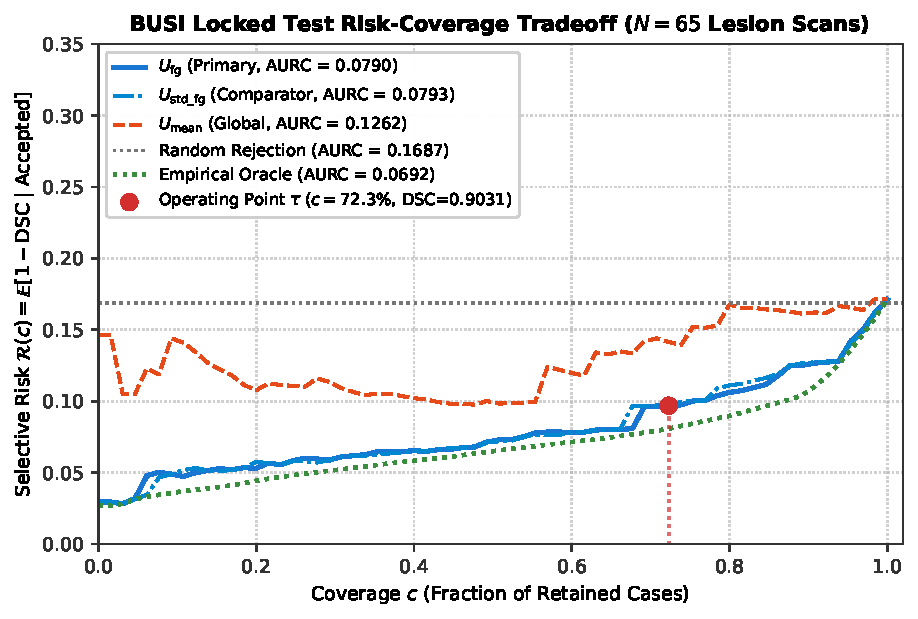
\includegraphics[width=\columnwidth]{fig4_busi_risk_coverage.pdf}
\caption{\textbf{Risk-coverage evaluation on the locked BUSI test lesion cohort ($N=65$).} Selective risk $\mathcal{R}(c) = \mathbb{E}[1 - \mathrm{DSC} \mid \mathrm{Accepted}]$ as a function of retained coverage $c$. $U_{\mathrm{fg}}$ (AURC $0.0790$) tracks close to the Empirical Oracle upper bound ($0.0692$) and decisively outperforms global averaging $U_{\mathrm{mean}}$ ($0.1262$) and uniform Random rejection ($0.1687$). The primary operating point ($\tau = 0.064058$) achieves $72.3\%$ coverage at DSC $0.9031$.}
\label{fig:busi_rc}
\end{figure}

\subsection{Experiment D: External Domain Generalization Benchmark}
Without any model retraining, fine-tuning, or threshold adaptation, we applied the frozen threshold ($\tau = 0.064058$) directly to the four external datasets. As reported in Table~\ref{tab:master_results} and Figure~\ref{fig:cross_domain}:
\begin{itemize}
    \item \textbf{UDIAT ($N=25$, Spain):} Baseline DSC was $0.7467 \pm 0.2992$. Rejection filtered out $11$ low-quality scans ($56.0\%$ coverage), raising accepted DSC to \textbf{0.8747} ($+0.1281$ gain, $95\%$ CI $[+0.0325, +0.2569]$). $U_{\mathrm{fg}}$ realized an AURC of $0.1133$ vs. $0.1979$ for $U_{\mathrm{mean}}$.
    \item \textbf{BUID ($N=35$, Academic):} Baseline DSC rose from $0.7900$ to \textbf{0.8818} ($+0.0919$ gain, $57.1\%$ coverage). AURC was $0.1094$ for $U_{\mathrm{fg}}$ vs. $0.1708$ for $U_{\mathrm{mean}}$.
    \item \textbf{BUSUC ($N=122$, Multi-center):} Baseline DSC rose from $0.8430$ to \textbf{0.8982} ($+0.0551$ gain, $63.9\%$ coverage). AURC was $0.0916$ for $U_{\mathrm{fg}}$ vs. $0.1368$ for $U_{\mathrm{mean}}$.
    \item \textbf{BUSBRA ($N=282$, Brazil):} Baseline DSC rose from $0.7511$ to \textbf{0.8536} ($+0.1025$ gain, $95\%$ CI $[+0.0789, +0.1278]$, $44.7\%$ coverage). AURC was $0.1529$ for $U_{\mathrm{fg}}$ vs. $0.2078$ for $U_{\mathrm{mean}}$.
    \item \textbf{Pooled External Benchmark ($N=464$):} Evaluated across all $464$ external scans, the frozen threshold retained $238$ cases ($51.3\%$ coverage), raising pooled accuracy from $0.7780$ to \textbf{0.8718} DSC ($+0.0939$ absolute gain, $95\%$ CI $[+0.0775, +0.1113]$, $p < 0.001$). Retained NSD rose from $0.8203$ to \textbf{0.9088} ($+0.0885$ gain).
\end{itemize}

\textbf{Disambiguation of Pooled AURC:} The case-level global AURC across all $464$ pooled external scans was \textbf{0.1267} for $U_{\mathrm{fg}}$ (vs. $0.1864$ for $U_{\mathrm{mean}}$, $\Delta\mathrm{AURC} = -0.0597$, $p < 0.001$; Random $0.2216$; Oracle $0.1046$). This global rank metric differs from the sample-weighted average of per-dataset AURCs ($0.1314$) and unweighted macro AURC ($0.1168$), because global ranking tests calibration across institutions simultaneously.

\begin{figure}[t]
\centering
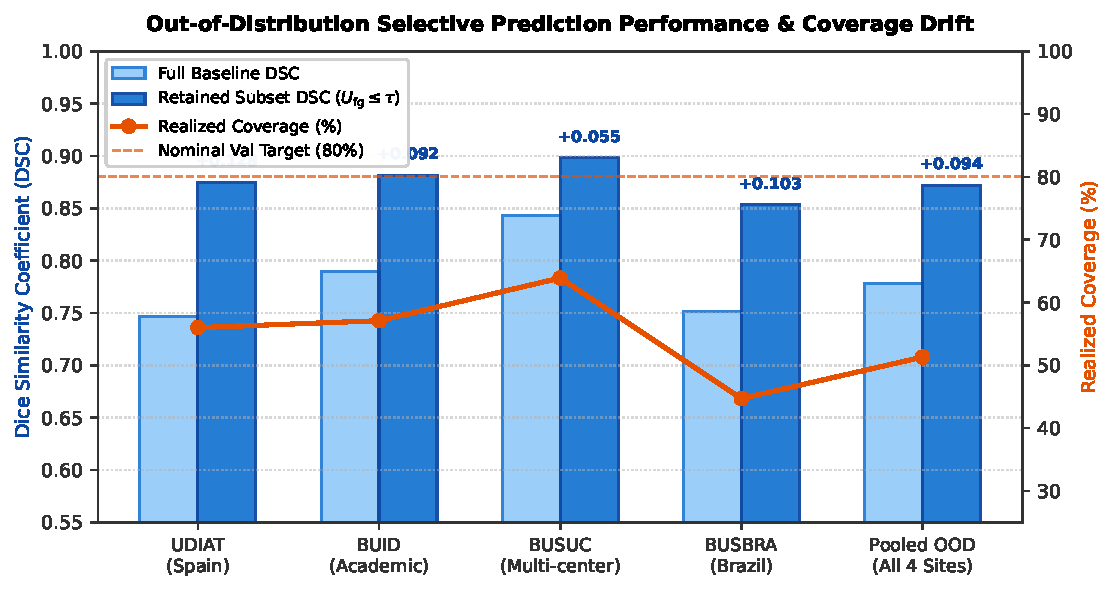
\includegraphics[width=\columnwidth]{fig5_cross_domain_performance.pdf}
\caption{\textbf{Out-of-distribution selective prediction performance and coverage drift across the four external benchmarks ($N=464$ cases).} Grouped bars compare baseline full-cohort DSC against retained subset DSC ($U_{\mathrm{fg}} \le \tau$). Selective prediction restores high accuracy ($>0.85$ DSC) across all external domains. The orange overlay depicts realized coverage, illustrating coverage drift from the nominal $80\%$ in-domain target down to $44.7\%$ on BUSBRA and $51.3\%$ pooled.}
\label{fig:cross_domain}
\end{figure}

\subsection{Experiment E: Failure Analysis and Safety Counterexamples}
To delineate the boundaries of uncertainty rejection, we audited individual failure modes:
\begin{enumerate}
    \item \textbf{Severe False-Certainty Failure Mode:} Figure~\ref{fig:qualitative_cases} (Row 3) illustrates case \texttt{116\_malignant.png} from the BUSI test split. The model produced a severely distorted segmentation ($\mathrm{DSC} = 0.2193$, $\mathrm{NSD} = 0.2393$) by erroneously expanding into posterior acoustic shadowing. Because the internal probability across this uniform dark region was falsely confident, foreground entropy remained low ($U_{\mathrm{fg}} = 0.06279 < \tau = 0.064058$). Consequently, the image bypassed rejection and was accepted into the autonomous partition. This counterexample directly falsifies the claim that uncertainty rejection can guarantee the detection of all severe segmentation failures.
    \item \textbf{Coverage Drift Under Domain Shift:} While the operating point $\tau = 0.064058$ was calibrated for $80.0\%$ coverage on BUSI validation, realized coverage dropped to $72.3\%$ on BUSI test, $56.0\%$ on UDIAT, $57.1\%$ on BUID, $63.9\%$ on BUSUC, and $44.7\%$ on BUSBRA (pooled external coverage: $51.3\%$). This demonstrates that acoustic domain shifts systematically elevate predictive entropy distributions, causing static thresholds to drift toward higher referral rates.
\end{enumerate}

\section{Discussion}

\subsection{The Mechanism of Selective Improvement}
A fundamental question in selective prediction is why accepted-case DSC increases so substantially ($+0.0939$ across $464$ OOD cases) when the model's segmentation weights remain completely unchanged. The mechanism is governed by the law of total expectation:
\begin{equation}
\mathbb{E}[\mathrm{DSC}] = c \cdot \mathbb{E}[\mathrm{DSC} \mid g=1] + (1 - c) \cdot \mathbb{E}[\mathrm{DSC} \mid g=0]
\end{equation}
Selective prediction does not repair defective segmentation masks. Rather, ranking images by $U_{\mathrm{fg}}$ concentrates poor segmentations into the rejected partition ($\mathbb{E}[\mathrm{DSC} \mid g=0] = 0.6791$), shifting the conditional mean of retained cases upward ($\mathbb{E}[\mathrm{DSC} \mid g=1] = 0.8718$) at the operational cost of human referral workload ($1 - c = 48.7\%$).

\subsection{Quality versus Workload Tradeoff}
The clinical deployment of selective prediction involves a tradeoff between automated throughput and diagnostic accuracy. On BUSBRA, achieving a retained DSC of $0.8536$ required referring $55.3\%$ of scans to expert sonographers. Deploying clinics must evaluate whether their staffing capacity supports such referral volumes. If a clinic requires a fixed referral workload (e.g., exactly $20\%$ referred), operating thresholds must be dynamically recalibrated to the specific scanner distribution.

\subsection{Ranking Quality vs. Calibrated Error Guarantees}
Our findings demonstrate that while $U_{\mathrm{fg}}$ provides an effective relative ranking of segmentation quality (Spearman $\rho = -0.7202$, AURC $0.0790$), it does not represent a calibrated probability of failure. The presence of false-certainty failures (e.g., \texttt{116\_malignant}) proves that deep networks can generate confident wrong segmentations in regions lacking high-frequency acoustic texture.

\section{Limitations and Methodological Constraints}
We explicitly record the limitations of this study:
\begin{enumerate}
    \item \textbf{Patient Provenance and Clustering:} Verified longitudinal medical record patient IDs are absent across all five public breast ultrasound benchmarks. In BUSBRA, filenames encode a heuristic prefix \texttt{bus\_XXXX-[l|r|s].png}, revealing $262$ unique patient/exam clusters across the $282$ test images ($20$ clusters contain bilateral scans). For BUSI, UDIAT, BUID, and BUSUC, patient identity is completely unknown. Consequently, our bootstrap confidence intervals reflect image-level resampling uncertainty rather than patient-clustered variation.
    \item \textbf{Pixel-Grid Spatial Spacing:} DICOM metadata containing physical pixel spacing (mm/pixel) is stripped from public releases. NSD was computed assuming isotropic pixel coordinates with tolerance $\tau=2$ pixels, which cannot be converted to physical millimeters.
    \item \textbf{Unexercised Empty-Mask Branch in OOD:} Across all $464$ external OOD images, MedCLIPSeg predicted at least one foreground pixel ($|\Omega_{\mathrm{fg}}| > 0$). Consequently, the second-stage empty-mask fallback gate ($U_{\mathrm{mean}} \le 10^{-4}$) was not empirically exercised in the OOD setting.
    \item \textbf{Static Threshold Sensitivity:} As demonstrated by coverage drift, a single fixed threshold cannot guarantee uniform clinical referral workloads across diverse scanner hardware.
\end{enumerate}

\section{Conclusion}
This study investigated uncertainty-based selective prediction for text-guided medical image segmentation under domain shift using a frozen MedCLIPSeg foundation model. We demonstrated that foreground-averaged predictive entropy ($U_{\mathrm{fg}}$) mathematically and empirically eliminates the background dilution effect that severely degrades global spatial averaging. Strictly calibrated on in-distribution validation data, the frozen operating threshold reliably triages segmentation outputs, elevating retained accuracy from $0.7780$ to $0.8718$ DSC across $464$ multi-center external scans. However, we also demonstrated that static operating points undergo substantial coverage drift under domain shift, and identified catastrophic false-certainty failure modes. These findings establish that while training-free selective prediction significantly enhances the reliability of automated medical segmentation, safe clinical deployment requires monitoring coverage drift and maintaining human oversight for ambiguous diagnostic presentations.

\section*{Acknowledgment}
This work was completed as part of the final research project for ELEC 6661 (Medical Image Processing, Fall 2026) at Concordia University, supervised under the IMPACT Lab (Prof. Hassan Rivaz and Omid Nejati Manzari). We acknowledge the open-source release of MedCLIPSeg by Koleilat et al. (CVPR 2026).

\bibliographystyle{IEEEtran}
\bibliography{references}

\end{document}
